% !TEX root = ../gnss_interference_resistant_thesis.tex
\documentclass[main.tex]{subfiles}

\begin{document}

\subsection{Spindulio formavimo įgyvendinimas}\label{sec:beamforming_concept}

Spindulio formavimui pasirinktas antenų masyvas sudarytas iš 4 antenų, išdėliotų
sta\-čia\-kam\-pio formoje, tarp kurių atstumas yra $l=\lambda / 2$. Toks
išdėstymas pasirinktas dėl galimybės formuoti spindulius dvejose plokštumose,
norint nutaikyti antenų maksimumą į kiekvieną GPS palydovą.
Atliekant spindulio formavimą, bus užtikrinama, kad atėjęs signalas yra
tiesioginis iš palydovo, o ne, pavyzdžiui, atsispindėjęs nuo šalia esančio pastato.

Norint žinoti nutaikymo kampą, reikia žinoti imtuvo poziciją, antenų pokrypį,
ir į kurią pasaulio šalį jos yra nusuktos, taip pat palydovų padėtį.
Dėl paprastumo šiame darbe,
bus laikoma, kad antenos visada nusuktos ta pačia kryptimi (šiaurės)
ir jos bus lygiagrečios su žemės paviršiumi. Pridėjus IMU (angl. Inertial Measurement
System), galima pamatuoti antenų pavirtimo kampus ir kompensuoti signalų apdorojime.

\begin{figure}[h]
    \begin{centering}
    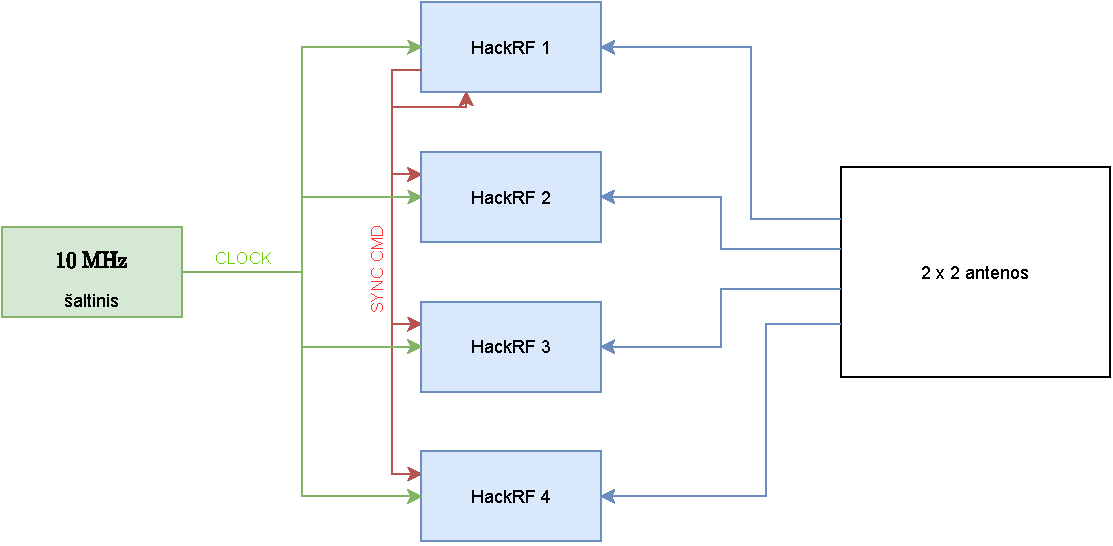
\includegraphics[scale=0.8]{drawings/beamformer_diagram}
    \par\end{centering}
    \protect\caption{\label{fig:gnss_beamform_block}Trikdžiams atsparaus GNSS imtuvo schema.}
\end{figure}

Imtuvo struktūra (\ref{fig:gnss_beamform_block}~pav.) pasirinkta pilnai skaitmeninė,
kad būtų sudaryta galimybė turėti daugumą
spindulių lygiagrečiai. Visi imtuvai naudoja tą patį taktinį dažnį, bei turi sujungtą
sinchronizacijos signalą. Toks sujungimas, kaip aptartas \ref{sec:hackrf} skyriuje,
užtikrina laikinę ir dažninę sinchronizaciją. Fazinė sinchronizacija turės būti
kalibruojama prieš kiekvieną matavimą, kadangi visi SDR maišytuvai naudoja lokalius
taktinio dažnio šaltinius, kurie yra generuojami naudojant PLL, kurių fazės
įjungimo metu yra atsitiktinės.

\begin{figure}[h]
    \begin{centering}
    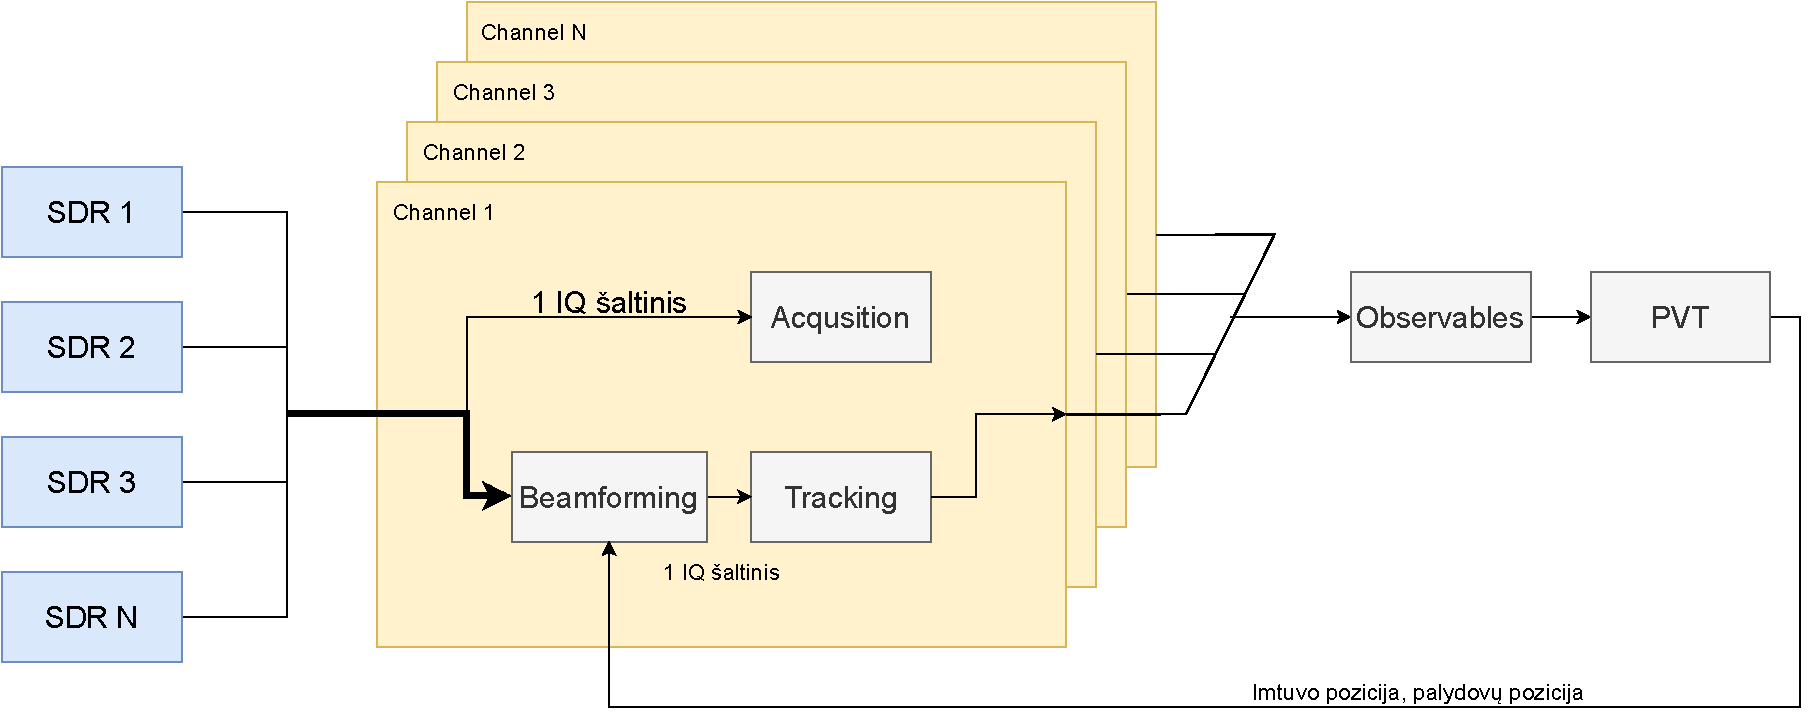
\includegraphics[scale=0.5]{drawings/beamformer_sw_implementation}
    \par\end{centering}
    \protect\caption{\label{fig:sw_beamformer_block}GNSS SDR blokinė diagrama, su pridėtu spindulio formavimu.}
\end{figure}

\ref{fig:sw_beamformer_block}~pav. pavaizduota siūloma GNSS SDR signalo apdorojimo
struktūra,
su integruotu spindulio formavimu. Didžiausias pakeitimas bus atliekamas
imtuvo kanaluose. Kiekviename kanale yra integruotas spindulio formavimo
blokas, kuris iš N (antenų skaičius) duomenų srautų padaro 1 duomenų
srautą. Tai bus atliekama, keičiant įėjimo signalų fazes ir juos
sudedant. Spindulio kryptis bus nustatoma iš PVT sugeneruotų duomenų:
imtuvo pozicijos, laiko ir palydovų orbitų.
Spindulio formavimas negalės būti pradedamas, kol nebus gauta pirminė
imtuvo pozicija, todėl tuo metu bus naudojamas signalas iš vienos antenos.


\end{document}
